\subsubsection{Computer Vision for Approach and Tracking Phases}
%
% Nassir
%
% describe CV method, refer to existing references
% provide analysis to explain why CV fails, with reference to experiemental data (image sequences)
The visual pose estimation is based on work of~\cite{Drummond2002} which relies on a known object geometry. The algorithm consisits of sampling model contours and edge detection, followed by a local optimization of the 3D rigd-body transform. The re-projection error is then minmized between visible model contour and image edges using Levenberg-Marquardt algorithm.
 %Related to this model matching approach is moving edges method~\cite{Comport2004} which differs from the former in contour samply strategy. The latter samples model contours in 2D, after projecting model lines on the image. These two approaches have their own advatnages and disadvantages which have been explored in~\cite{Comport2005}. While both approaches show similar performance, the former is easier to implement as it presents a direct and accurate formulation for minimizing the reprojection error from %3D to 2D~\cite{Oumer2015}. 
The complex motion trajectory (tumbling and an abrupt change of angular velocity) of the target poses difficulty in visual tracking. In order to address this problem, a motion prediction scheme based on the extended kalman filter CHECK is integrated into the local optimization. The prediction relies on a simple kinematic motion model assuming constant frame to frame motion. Under this assumption, the visual tracker is able to cope with relatively higher image motion between two camera frames. Moreover, the short-term prediction scheme helps the visual tracker reduce the search space in order not to trap in potential local optima during minimization of the cost function. The qualitative tracking results are illustrated in Fig.~\ref{fig:TrackingImages}, with examplar tracked images during the approach and tracking phases. Those in red indicate the projections of model contours onto the image edges at the estimated pose. The axes of the coordinate frame of the grasping point are indicated in red, green and blue. The overlap of the model contours and image edges shows the successful tracking and pose estimation.
%
%\begin{figure}
%\centering
%\begin{subfigure}
%	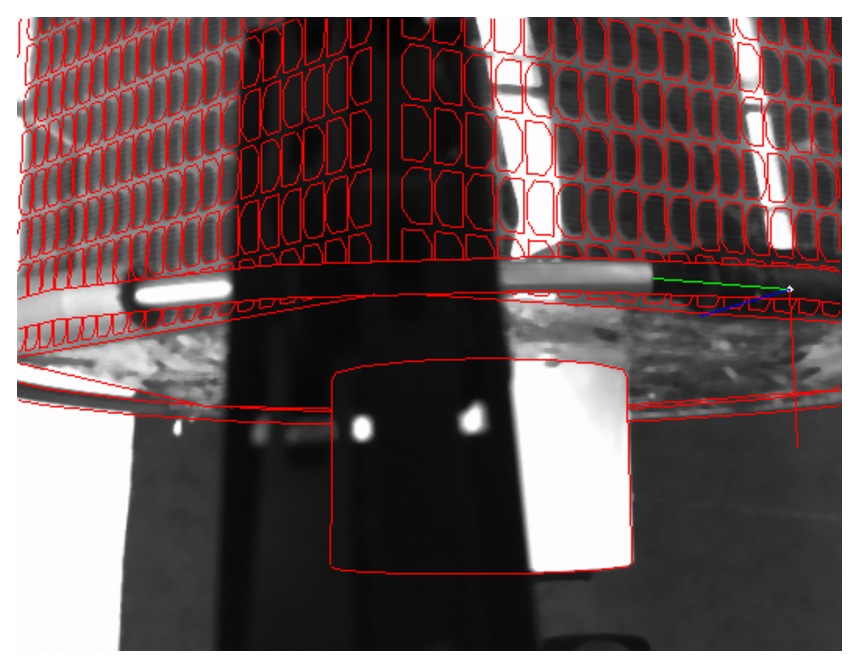
\includegraphics[angle=0,width=0.95\textwidth]{./figures/frame0786_result_cam0}
%	\caption{approach}
%\end{subfigure}
%\begin{subfigure}
%	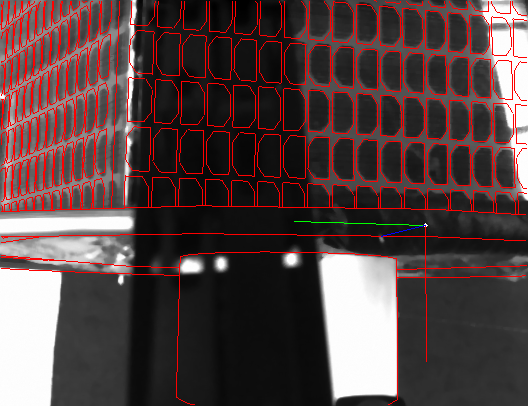
\includegraphics[angle=0,width=0.95\textwidth]{./figures/frame0849_result_cam0}
%	\caption{Tracking}
%\end{subfigure}
%\begin{subfigure}
%	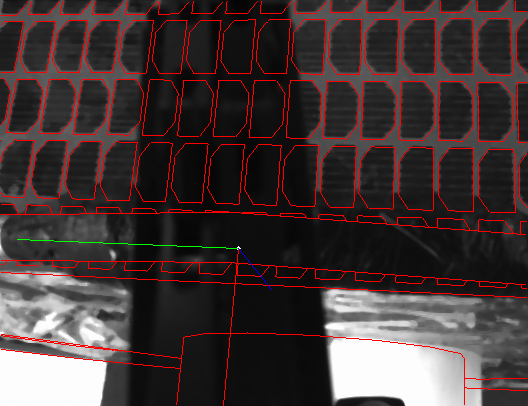
\includegraphics[angle=0,width=0.95\textwidth]{./figures/frame0922_result_cam0}
%	\caption{Tracking}
%\end{subfigure}
%\begin{subfigure}
%	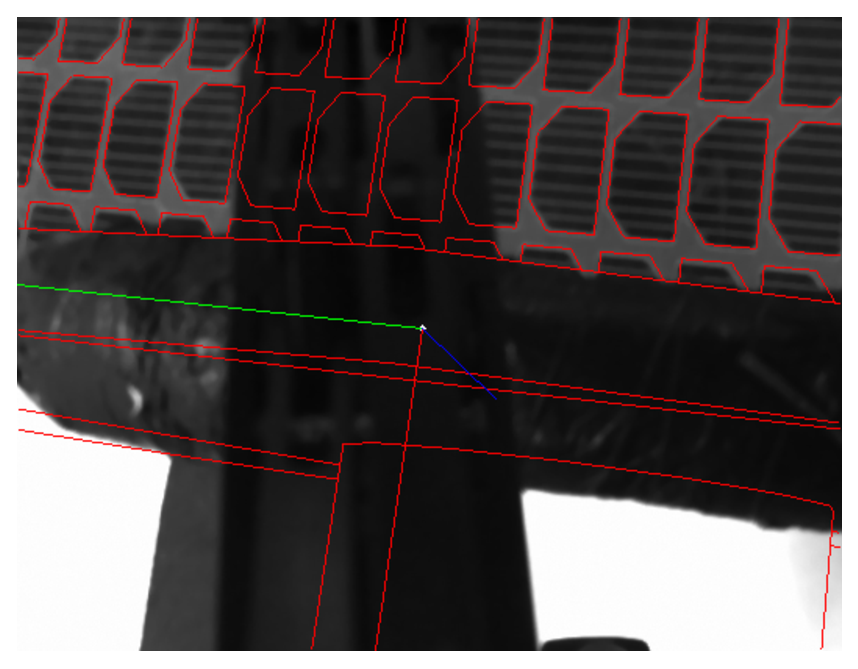
\includegraphics[angle=0,width=0.95\textwidth]{./figures/frame0954_result_cam0}
%	\caption{Tracking}
%\end{subfigure}
%\label{fig:TrackingImages}
%\caption{Exemplar images during visual tracking for approach and tracking phase. The overlay of the model contours and image edges shows the successful tracking and pose estimation. The %target features reduce significantly as the manipulator approaches close to grasping. The axes of the coordinate frame of grasping point is indicated in red, green and blue }
%\end{figure}


%
\begin{figure*}
\centering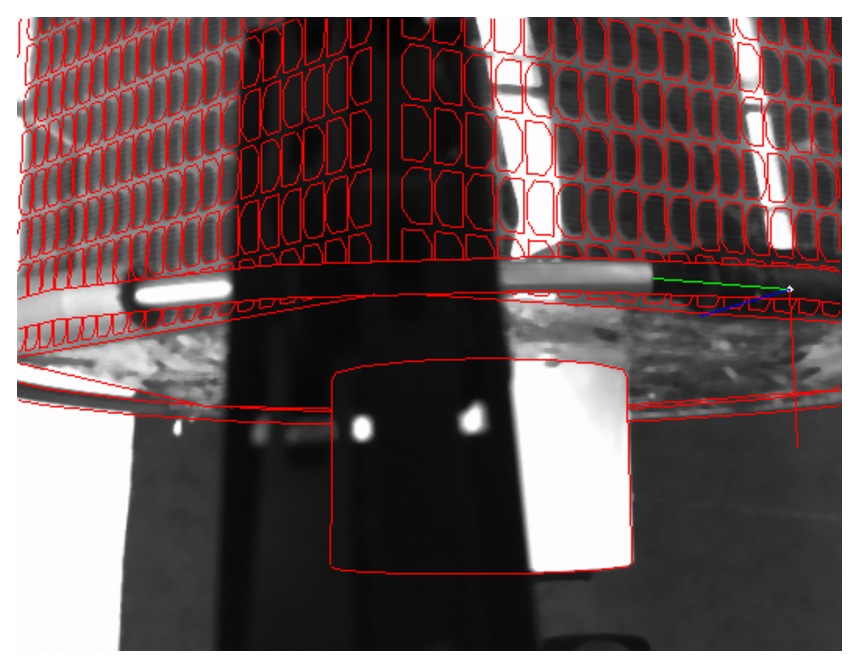
\includegraphics[angle=0,width=0.24\textwidth]{./figures/frame0786_result_cam0}
\centering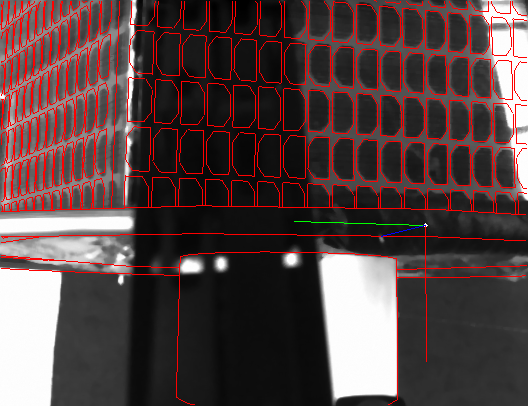
\includegraphics[angle=0,width=0.24\textwidth]{./figures/frame0849_result_cam0}
\centering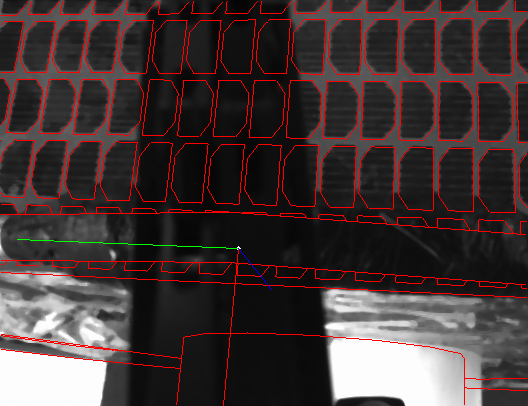
\includegraphics[angle=0,width=0.24\textwidth]{./figures/frame0922_result_cam0}
\centering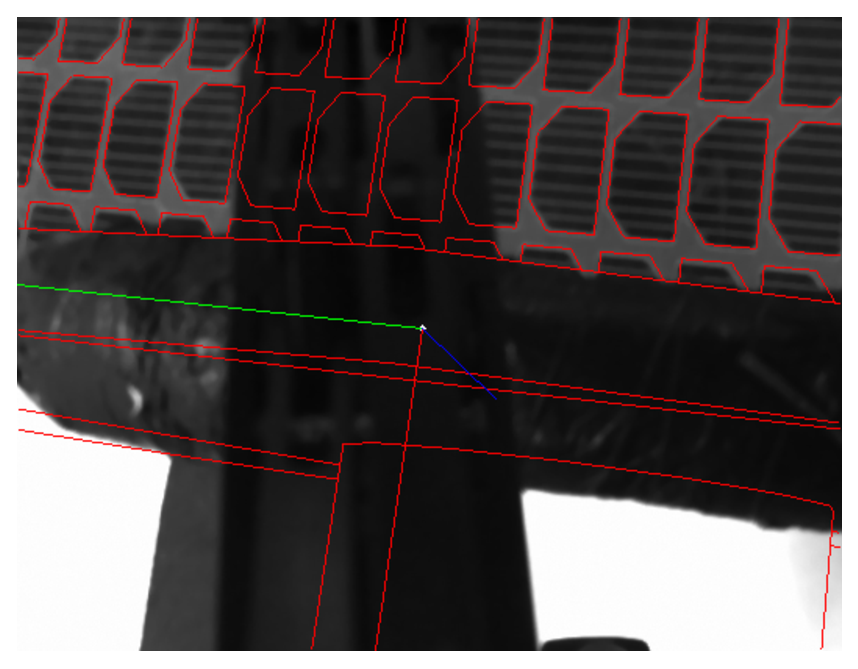
\includegraphics[angle=0,width=0.24\textwidth]{./figures/frame0954_result_cam0}
\caption{Exemplar images during visual tracking for approach and tracking phase. The overlay of the model contours and image edges shows the successful tracking and pose estimation. The axes of the coordinate frame of grasping point is indicated in red, green and blue. The target features reduce significantly at very close range because of gripper finger occlusion (black in the image) and camera field of view.}
\label{fig:TrackingImages}
\end{figure*}


%There exist, however a few cases where the visual tracking was not able to provide the required pose accuracy for the visual servoing. For example, the inherent vision-based %pose estimation problem assocociated to in-plane motion where lateral rotation estimation error is large, particularly when a partial surface of the target with planar geometry is momentarily visible in non perspective view. Moreover, the outliers due to occlusion and limited field of view poses tracking failure particularly at very close range, as shown in Fig.~\ref{fig:GraspingImages}. Fortunately, at this range the gripper is a few millimeters from the grasping point, hence the implemented motion predictor supports final grasping phase.

%\begin{figure}
%\centering
%\begin{subfigure}
%	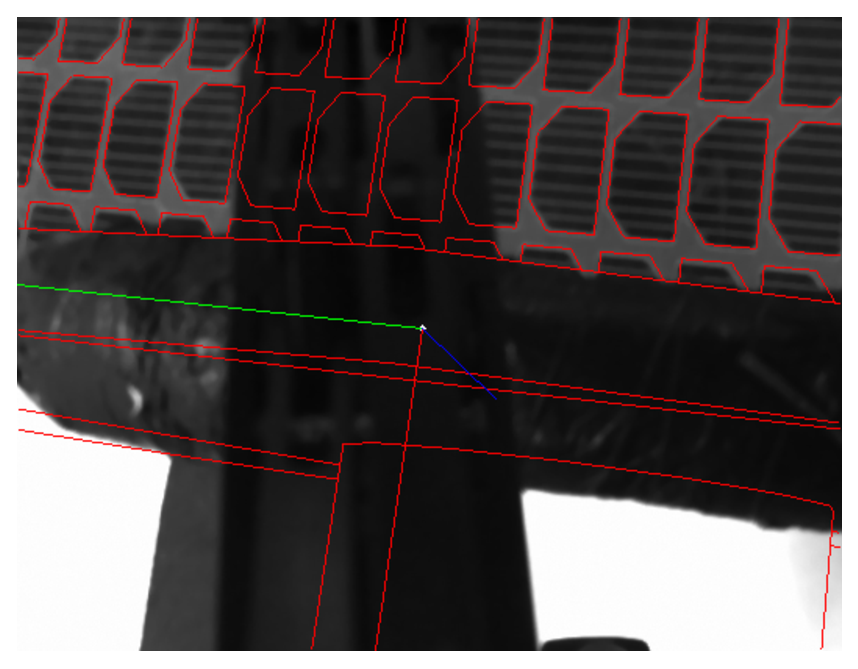
\includegraphics[angle=0,width=0.95\textwidth]{./figures/frame0954_result_cam0}
%	\caption{approach}
%\end{subfigure}
%\begin{subfigure}
%	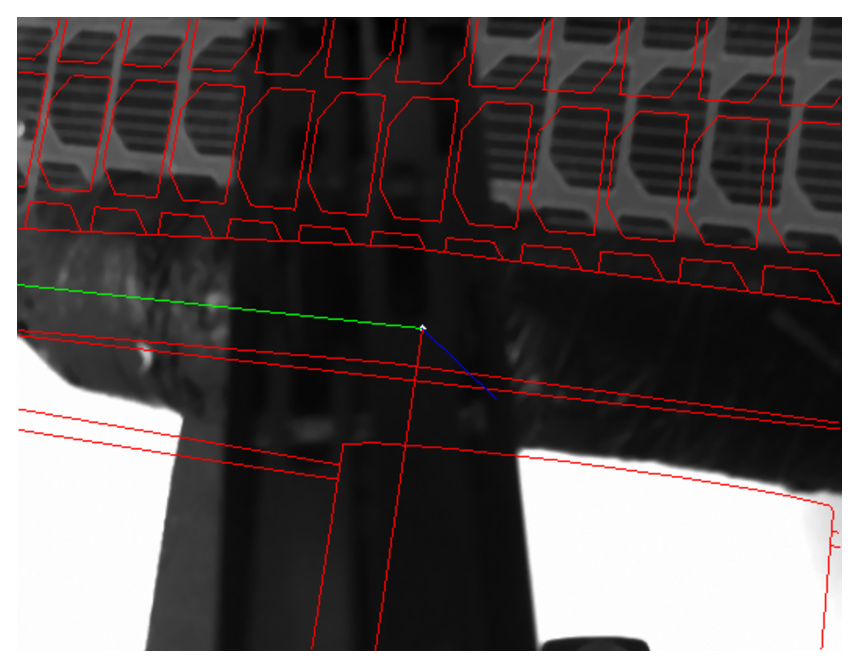
\includegraphics[angle=0,width=0.95\textwidth]{./figures/frame0955_result_cam0}
%	\caption{Tracking}
%\end{subfigure}
%\begin{subfigure}
%	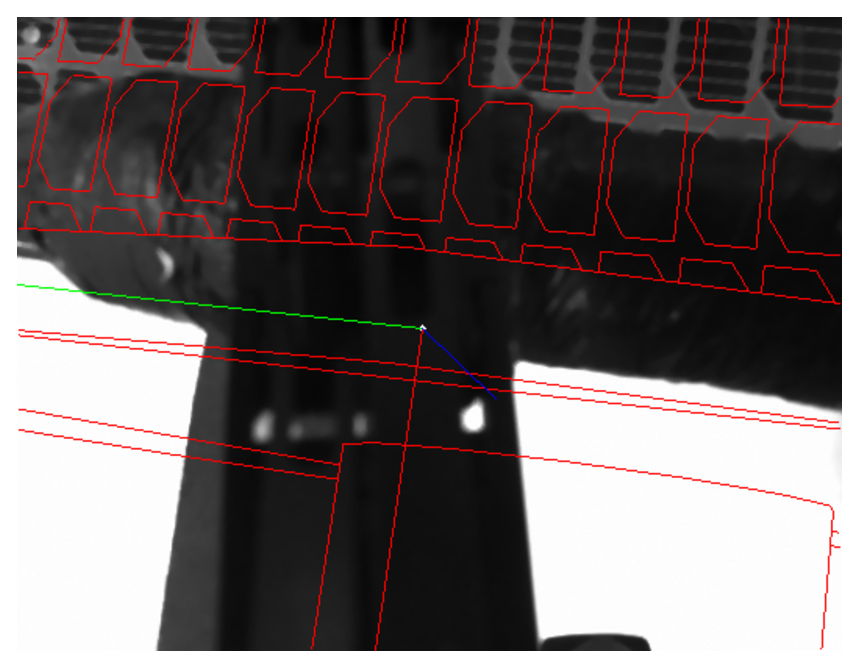
\includegraphics[angle=0,width=0.95\textwidth]{./figures/frame0956_result_cam0}
%	\caption{Tracking}
%\end{subfigure}
%\label{fig:GraspingImages}
%\caption{Failure cases of the visual tracking. At very close range, the visible target features are not sifficient for pose estimation because of occlusion (black in the images) and  %reduced field of view}
%\end{figure}

%\begin{figure*}
%\centering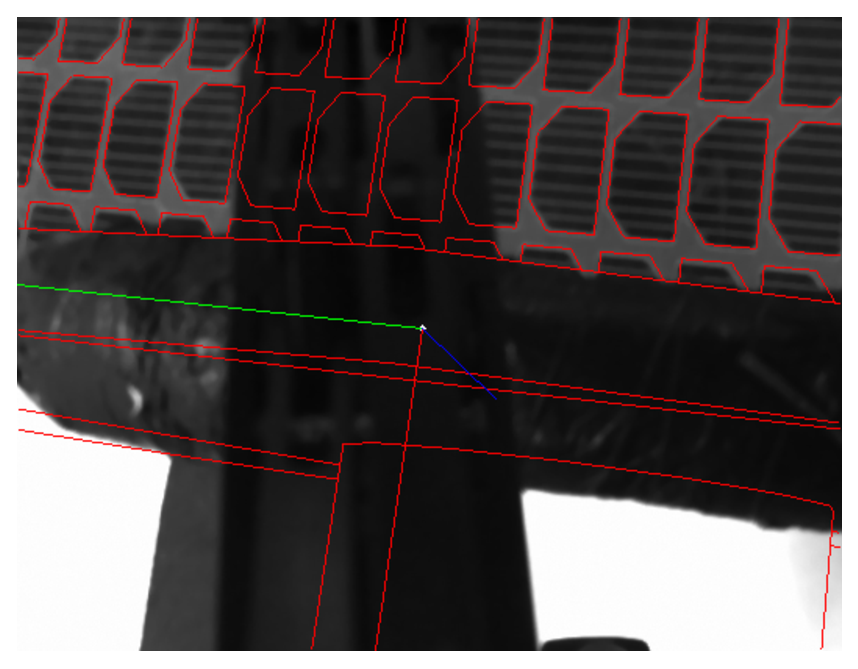
\includegraphics[angle=0,width=0.24\textwidth]{./figures/frame0954_result_cam0}
%\centering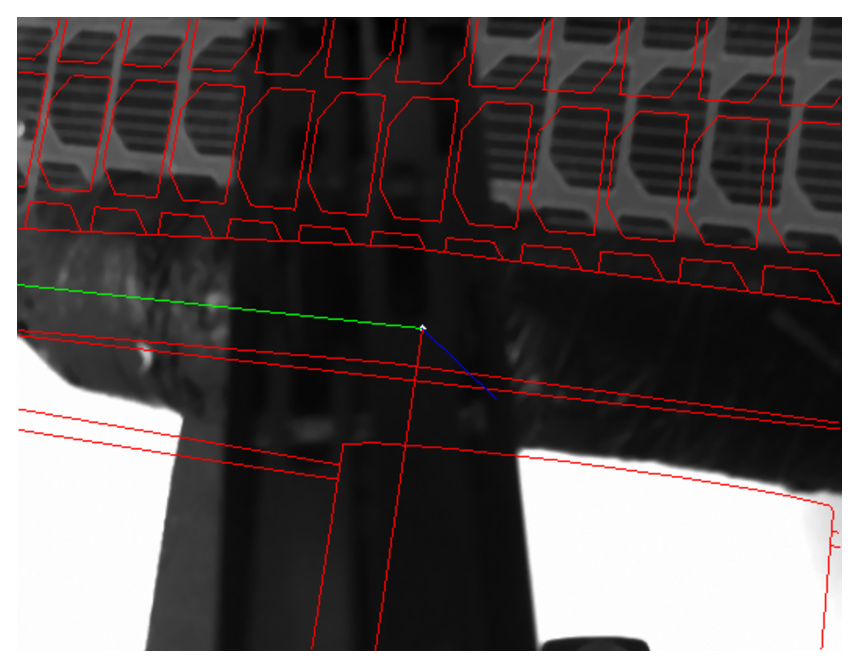
\includegraphics[angle=0,width=0.24\textwidth]{./figures/frame0955_result_cam0}
%\centering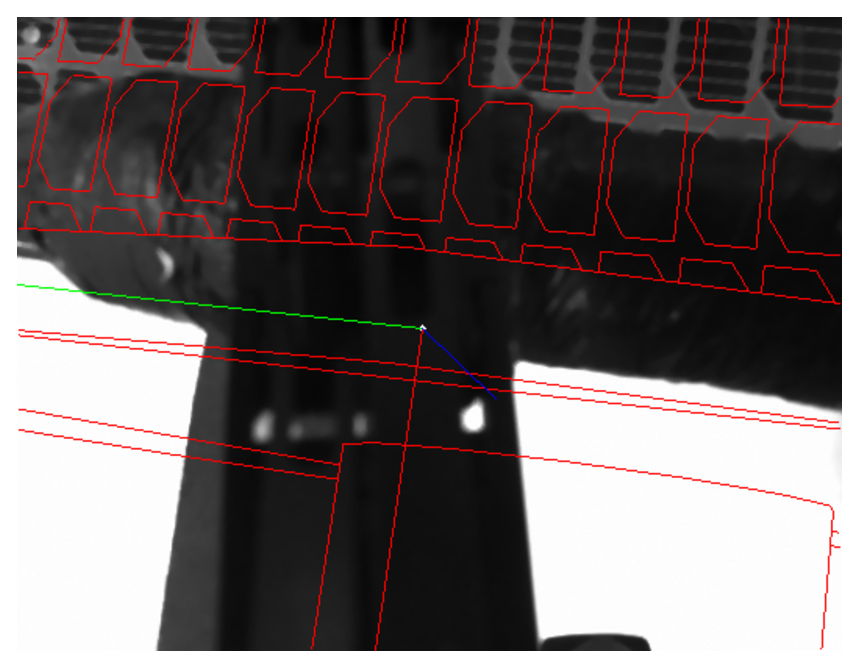
\includegraphics[angle=0,width=0.24\textwidth]{./figures/frame0956_result_cam0}
%\caption{Failure cases of the visual tracking. At very close range, the visible target features are not sifficient for pose estimation because of occlusion (black in the images) and  reduced field of view.}
%\label{fig:GraspingImages}
%\end{figure*}

% ---- You may menstion this in future work section-----
%In the future, the performance of the visual tracking will be improved, addressing problems related to in-plane motion, local minima and large image pixel velocity by integrating dynamic motion model of the coupled satellite-manipulator system for long-term prediction. Moreover, the visual tracking will be validated in a representative space environment with proper lighting conidtion as in~\cite{OumerPhdThesis}.

%	i. The visual servo also includes a pose estimation algorithm, which relies on a predefined simplifies model of the Target - show image with simplified model of the target

%
\subsection{Joint Tracking Control for Stabilization Phase}
%
% Roberto or Marco
% Describe tracking controller
% 
The tracking controller for the rigidization phase is described in Fig.~\ref{fig:blockdiagram}. The motion synthesizer provides an input expressed as $q_ref. \dot{q}_{ref}$. The control law for the tracking controller adopted here is then as follows
\begin{equation}
\MatO{\tau}{}_{rig} = \MatO{K}{}_{p} (q_{ref}-q) + \MatO{K}{}_{d} (\dot{q}{}_{ref}-\dot{q})
\label{eq:rigidiz_control}
\end{equation}
where $\MatO{K}{}_{p}$ and $\MatO{K}{}_{d}$ are (7x7) diagonal matrices including the stiffness and damping gains respectively. The first proportional term plays an inportant role, since itbrings the system into a feasible final configuration, as dictated by the motion planner. 
%
\section{Experimental facility}
% Roberto
%	i. introduce falicity
%	ii. describe extensions: target motion, post-grasping tumbling motion
%	iii. 4N/1Nm (CHECK) deadband in Target FTS - removed after grasping
%	iv. End-effector pads to avoid slipage (?)
%
The OOS-SIM experimental facility is described in detail in~\ref{jordi}. Some new features were implemented to perform the grasping task of a rotating Target. The motion of the Target was allowed in all of its six degrees of freedom, by means of the online integration of its equations of motion (single rigid body) and the input to this from a force/torque sensor at the base of the Target mockup. Due to the sensor noise and to uncertainty in the gravity compensation of the sensor signal for the mockup weight (approx. 30 kg), a deadband filter was used in the approach and tracking phase in all three Cartesian directions. The filter was however removed at the moment of gripper closure and for the subsequent rigidization phase.

In order to simulate the motion of the two satellites after the grasp, a master-slave approach was used, in which the Target followed the Light-Weight Robot through the internal actions which the latter imparted on it. The Chaser instead was commanded by the online integration of the equations of conservavation of linear and angular momentum of the multibody system consisting of the Chaser and the robot manipulator:
\begin{equation}
\MatO{L}{}_{C}(\MatO{V}{}_{e}) + \MatO{L}{}_{LWR}(\MatO{V}{}_{e}, \MatO{q}, \MatO{\dot{q}}) = \MatO{L}{}_{T}(\MatO{V}{}_{t}),
\label{eq:angmom}
\end{equation}
where $\MatO{L}{}_{C}$, $\MatO{L}{}_{LWR}$ and $\MatO{L}{}_{T}$ are the momentum of the Chaser, of the Light-Weight Robot and of the Target respectively. Note in fact, that the left-hand side is zero before the grasp. After the grasp, the inertial parameters of the robot end-effector are updated to include those of the Target, in function of the measured relative pose with respect to it. As such, the total momentum remains constant and Eq.~(\ref{eq:angmom}) can be solved for the twist of the Chaser $\MatO{V}{}_{e}$ and integrated in time to obtain its pose $\MatO{H}{}_{e}$.
%
\section{Results}
%
% 1 pp
%
\begin{figure}[t!]
\psfrag{qd}[cc][cc][\FontFigB]{$\MatO{\dot{q}}$ [deg/s]}
\psfrag{t}[cc][cc][\FontFigB]{$t$ [s]}
\centering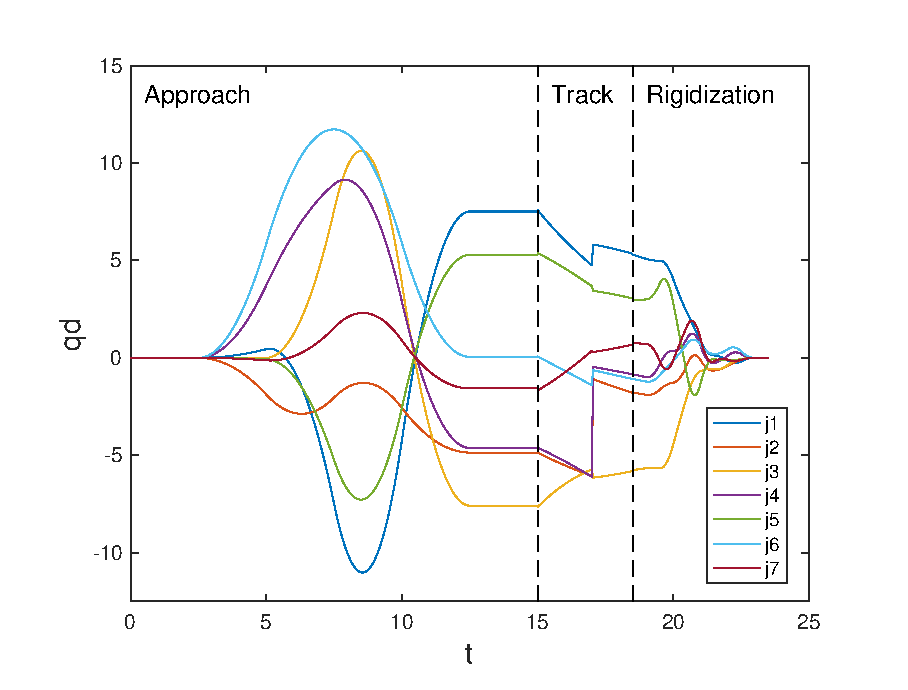
\includegraphics[angle=0,width=0.42\textwidth]{./figures/Joint_vel_2degs}
\caption{Simulated robot manipulator joint velocities for a Target spin velocity of 2 deg/s.}
\label{fig:Joint_vel_2degs}
%\vspace{-10pt}
\end{figure}
%
Fig.~\ref{fig:Joint_vel_2degs} shows the motion planner solution for a Target spin velocity of 2 deg/s. The figure shows the three phases of the maneuver. The transition from the approach to the tracking phase is smooth, as the end-effector alligns itself with the grasping point on the Target. The values of the parameters $\phi_{e \: mid}$ and $\phi_{e \: delta}$  was set to 40 and 7.5 deg respectively. The tracking phase lasts 3.5 seconds to allow for the gripper to close onto it. The rigidization phase lasts five seconds and the number of parameters per joint was $N_B=6$. The solution resulted from a global search,  which found different local minima, as expected, due to nonlinearity of the optimization problem. 

The control gains were defined as ... $K_p$, $K_d$, nullspace K. The deadband filter of the Target force/torque sensor signals were set to 4N and 1Nm.

%
\begin{figure}[t!]
\psfrag{q}[cc][cc][\FontFigB]{$\MatO{\Delta{q}}$ [deg/s]}
\psfrag{t}[cc][cc][\FontFigB]{$t$ [s]}
\centering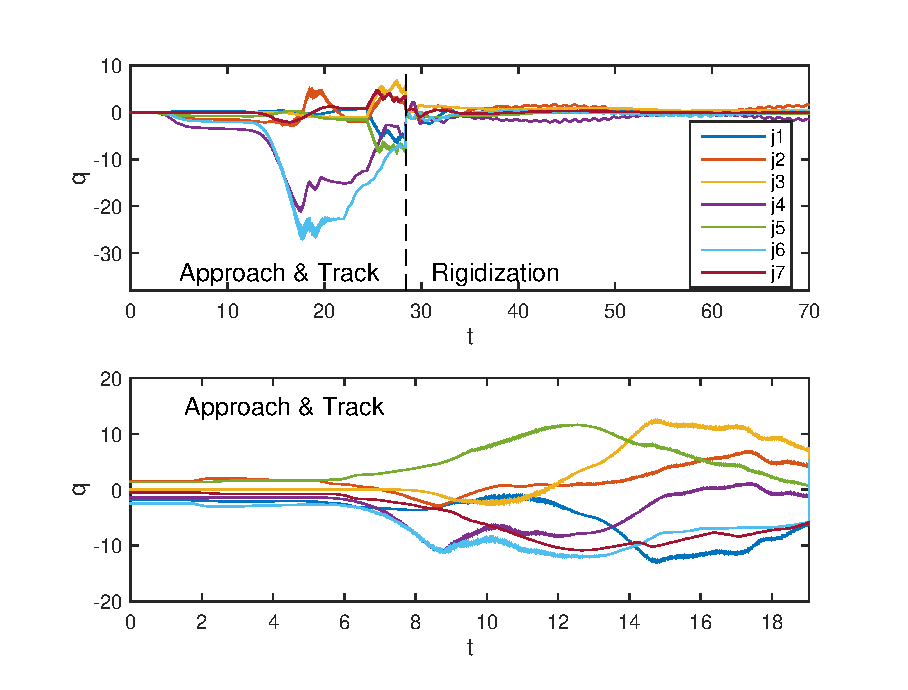
\includegraphics[angle=0,width=0.42\textwidth]{./figures/joint_space_motion_2subplots}
\caption{Measured robot manipulator joint position error for Target spin velocity of 1 deg/s (top) and 2 deg/s (bottom). The the latter case only the approach phase is shown, in which however the use of the EKF and of the extended parameterization of the joint motion give a net increase in joint-space tracking performance.}
\label{fig:joint_space_motion_2subplots}
%\vspace{-10pt}
\end{figure}
%
%
\begin{figure}[t!]
\psfrag{xx
}[cc][cc][\FontFigB]{$\MatO{\omega}{}_{t}$ [deg/s]}
\psfrag{yy}[cc][cc][\FontFigB]{$\MatO{\phi}{}_{t}$ [deg/s]}
\psfrag{t}[cc][cc][\FontFigB]{$t$ [s]}
\centering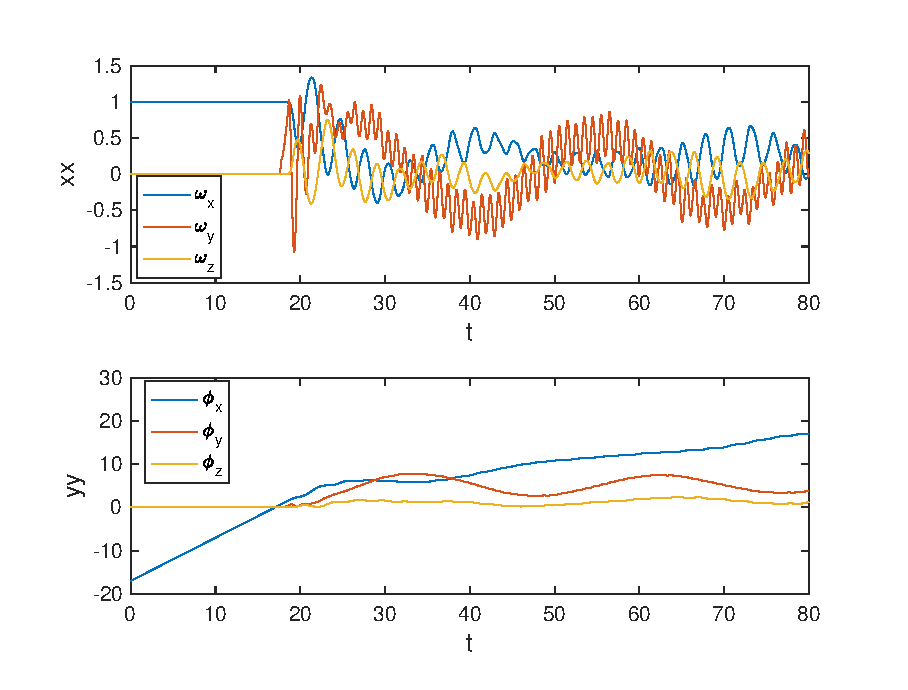
\includegraphics[angle=0,width=0.42\textwidth]{./figures/Target_motion}
\caption{Measured Target angular velocity (top) and orientation (bottom) for the 1 deg/s case. The post-grasping tumbling of the sattellite stack is visible in the (reduced) rotation about the $x$-axis.}
\label{fig:Target_motion}
%\vspace{-10pt}
\end{figure}
%

Fig.~\ref{fig:joint_space_motion_2subplots} shows the measured robot manipulator joint position error, defined as $\MatO{q}{}_{ref}-\MatO{q}$, for the cases of Target spin velocities of 1 deg/s and 2 deg/s respectively. In the experiments on the OOS-SIM facility it was in fact found that the rigidization task for the 2 deg/s case was intractable with the current setup, since the effacts of the time delay in the control loop are not yet accounted for (see~\ref{marco}). As such the experimental results presented here for the rigidization phase only relate to the 1 deg/s case. In Fig.~\ref{fig:Target_motion} the measurement of the Target motion is shown, in which the detrimental effect of the time delay is visible in the very slow damping of the angular velocity. 

Furthermore, the inertial parameters of the two satellites used in the facility model were increased with respect to ideal values. This was done in order to limit the velocities commanded to the industrial robots. The values taken here were.... chaser, target inertias, L

Returning to Fig.~\ref{fig:joint_space_motion_2subplots}, the error in the joint position is shown to improve substantially for the second case, due to the fact that the EKF and the joint motion parameterization shown in Fig.~\ref{fig:Joint_vel_2degs} is used (the manuever was not possible without these new features). While the first provides a soomther estimate of $\MatO{H}{}_{ge}$ (as shown below), the latter reduces the pixel velocity by a factor of two. At the point of transition between the tracking and the rigidization phase ($t=28$), the joint position error becomes zero, due to the recomputation of the reference trajectory (see Section\ref{sec:rigidization}). The tracking error in the rigidization phase is then shown to remain small.

Figures~\ref{fig:fig_norm_errors} and~\ref{fig:states_EKF} describe the EKF performance... say that new formulation is a lot better than the on in the literature.
%
\begin{figure}[t!]
\psfrag{y1}[cc][cc][\FontFigB]{$||\Delta r_c||^2$}
\psfrag{y2}[cc][cc][\FontFigB]{$||\Delta r_c||^2$}
\psfrag{leg1}[cc][cc][\FontFigS]{$EKF$}
\psfrag{leg2}[cc][cc][\FontFigS]{$Vision$}
\psfrag{x}[cc][cc][\FontFigS]{$EKF$}
\psfrag{y}[cc][cc][\FontFigS]{$Vision$}
\psfrag{t}[cc][cc][\FontFigB]{$t$[sec]}
\psfrag{ekf}[cc][cc][\FontFigS]{$EKF$}
\psfrag{vision}[cc][cc][\FontFigS]{$Vision$}
\centering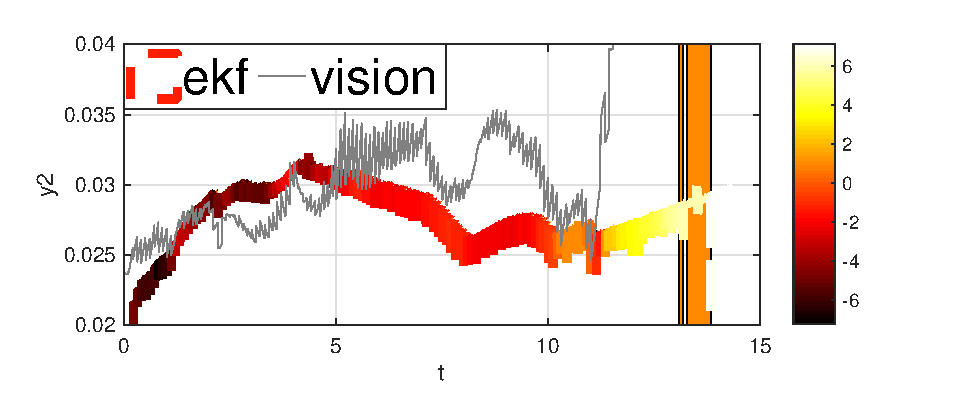
\includegraphics[angle=0,width=0.47\textwidth]{./figures/fig_norm_errors}
\caption{Comparison of direct-Vision measurements with EKF, based on the norm $||\Delta r_c^2||$. As $||r_c|| \rightarrow 0$, the statistical measure of fitness, $\chi^2 \rightarrow \infty $ eventually leading to pose estimation failures due to degenerate observability.}
\label{fig:fig_norm_errors}
%\vspace{-10pt}
\end{figure}
%
%
\begin{figure}[t!]
\psfrag{om}[cc][cc][\FontFigB]{$\omega$}
\psfrag{omhat}[cc][cc][\FontFigB]{$\hat{\omega}$}
\psfrag{true}[cc][cc][\FontFigB]{$\omega$}
\psfrag{t2}[cc][cc][\FontFigB]{$t$[sec]}
\psfrag{t1}[cc][cc][\FontFigB]{$t$[sec]}
\psfrag{qua}[cc][cc][\FontFigB]{$\mu$}
\psfrag{qhat}[cc][cc][\FontFigB]{$\hat{\mu_{EKF}}$}
\psfrag{vision}[cc][cc][\FontFigB]{$\mu_V$}
\centering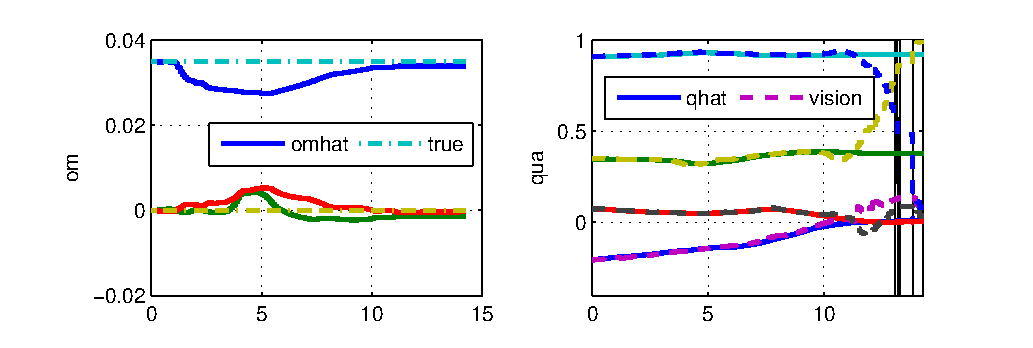
\includegraphics[angle=0,width=0.48\textwidth]{./figures/states_EKF}
\caption{a) Target state estimation ($\omega$) in EKF for tracking control. b) Divergence of visual tracking's orientation estimate towards end of maneuver.}
\label{fig:states_EKF}
%\vspace{-10pt}
\end{figure}
%
\section{Discussion and Conclusion}
%
The main achivement of this paper is to demonstrate the feasibility of a grasping strategy based on Target motion prediction [], robot motion planning [] and trajectory tracking, specifically for the latter step. In fact, due to modelling uncertainties, the reference trajectory has to be partially adapted online. A method is presented and validated here, which does that while favouring joint position related motion constraints. The tracking controller is then shown to succesfully perform the task. In this way, the fesible (and optimal) motion planning solutions computed offline, with much computational effort, are shown to be useful for control purposes. The reference trajectories are computed taking a complete three-dimensional multibody dynamics model into consideration, without simplifying assumptions.

We also argue that a reference trajectory based method provides greater robustness than local control methods. The control method must provide a guarantee that the grasping point can be tracked at all times and that the rigidization phase which follows remains feasible. Local control (e.g., potential) methods generally cannot provide this guarantee. Free-floating robots are known to possess dynamic singularities, which are function of the related distribution of its inertia. Their position in joint space, for the multibody system of interest here, is not only to the author's knowledge not representable, but is also variable in time during the robot's operations, due to changes in the inertial distribution. 

A second major achievement of this paper is the implementation of an Extended Kalman Filter which ensures a Lipschitz continuity of measurements, which makes the control method robust for executing the grasping task. It is in fact shown that the visual tracking algorithm adoped may become degenerate in the vicinity of the Target. Furthermore, the new formulation to reduce the computational footprint has been shown to give a signifcant improvement. Finally, given that the visual servo along with manipulator dynamics is known to lose passivity in presence of target motion [], the computation of the reference trajectory provides the necessary feedforward terms which ensure passivity unter the assumption of no modelling errors. This is complemented by the estimate of the Target velocity provided by the Kalman filter, as shown in Fig.\ref{fig:states_EKF}. As a result, the overall system is passive in the absence of external torques on the Target.

A limitation of the presented method is however also recognized. We argued, in fact, that the modelling uncertainties are small and as such, by grossly tracking the reference trajectory, the feasibility of the complete maneuver is guaranteed. In reality, the reference trajectory is only feasible at predefined via points along it, given the time discretization of the optimal control problem. This does not say anything about the feasibility of the solution in its vicinity. Future work will need to address this robustness issue, given that the tracking controller departs from the reference trajectory to account for the uncertainties. 

Future work will also be dedicated to improving the performance of the facility in the coupled configuration. Furthermore, the sensing of the Chaser, to include typical sensor noise and sampling times, will be considered.
%
%
%"In this way, by grossly tracking the reference trajectory the feasibility of the complete maneuver is guaranteed. As such, the end time of the stabilization phase need not be minimal, as suggested in [Aghili], since it is sufficient that the system remains in the vicinity of the planned trajectory, and may be chosen following a different cryterion. Minimum energy maneuvers can be considered as a viable alternative, since, as we will see, they are more robust to modelling errors and visual servo inaccuracies."
%
%Following target trajectory and slowing it down does not take account of chaser inertia. Providing a MBS solution vs Aghili's single rigid body solution.
%
%The satellite states are assumed to be ideal
%
%
%\section{Videos}
%1. simulation - bernhard
%2. facility
